% ---------------------------- DIFFERENCE ---------------------------- 

\begin{table*}[h]
\small\sf\centering
%
\caption{Cut-and-fill experiment: a participant sculpts the study landscape using Tangible Landscape's difference analytic, which shows where to add sand (blue) and remove sand (red).}
\vspace*{1em}
\ra{1.3}
\begin{tabular}{m{0.425\textwidth} m{0.425\textwidth}}
\includegraphics[width=0.425\textwidth]{images/experiments/difference_1.jpg} &
\includegraphics[width=0.425\textwidth]{images/experiments/difference_2.jpg}\\
\end{tabular}
\label{fig:diff} 
%
\vspace*{1.5em}
%
\caption{Cut-and-fill experiment: maps of raster statistics and geospatial analyses draped over a 3D rendering of the topography for all participants, 3D modeling novices, and 3D modeling experts.}
\vspace*{1em}
\ra{1.3}
\begin{tabular}{m{0.1\textwidth} m{0.2\textwidth} m{0.2\textwidth} m{0.2\textwidth} m{0.2\textwidth}}
\toprule
& \multicolumn{1}{c}{Elevation} & \multicolumn{1}{c}{Stdev.~ of differences} & \multicolumn{1}{c}{Slope} & \multicolumn{1}{c}{Landforms}\\
\midrule
%
Reference & 
\includegraphics[width=0.2\textwidth]{images/render_3d/3d_experts/dem_4.png} &
\includegraphics[width=0.2\textwidth]{images/render_3d/3d_experts/dem_difference_4.png}
&
\includegraphics[width=0.2\textwidth]{images/render_3d/3d_experts/slope_4.png} &
\includegraphics[width=0.2\textwidth]{images/render_3d/3d_experts/forms_4.png}\\
%
Mean & 
\includegraphics[width=0.2\textwidth]{images/render_3d/participants/mean_dem_4.png} &
\includegraphics[width=0.2\textwidth]{images/render_3d/participants/stdev_regression_difference_series_4.png} &
\includegraphics[width=0.2\textwidth]{images/render_3d/participants/mean_slope_4.png} &
\includegraphics[width=0.2\textwidth]{images/render_3d/participants/mean_forms_4.png}\\
%
3D novices & 
\includegraphics[width=0.2\textwidth]{images/render_3d/3d_novices/mean_dem_4.png} &
\includegraphics[width=0.2\textwidth]{images/render_3d/3d_novices/stdev_regression_difference_series_4.png} &
\includegraphics[width=0.2\textwidth]{images/render_3d/3d_novices/mean_slope_4.png} &
\includegraphics[width=0.2\textwidth]{images/render_3d/3d_novices/mean_forms_4.png}\\
%
3D experts & 
\includegraphics[width=0.2\textwidth]{images/render_3d/3d_experts/mean_dem_4.png} &
\includegraphics[width=0.2\textwidth]{images/render_3d/3d_experts/stdev_regression_difference_series_4.png} &
\includegraphics[width=0.2\textwidth]{images/render_3d/3d_experts/mean_slope_4.png} &
\includegraphics[width=0.2\textwidth]{images/render_3d/3d_experts/mean_forms_4.png}\\
%
& 
\multicolumn{1}{c}{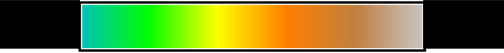
\includegraphics[width=0.2\textwidth]{images/legends/elevation_legend_4.pdf}} &
\multicolumn{1}{c}{\includegraphics[width=0.2\textwidth]{images/legends/stdev_diff_legend.pdf}} &
\multicolumn{1}{c}{\includegraphics[width=0.2\textwidth]{images/legends/slope_legend.pdf}} &
\multicolumn{1}{c}{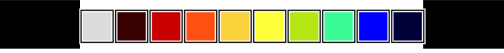
\includegraphics[width=0.2\textwidth]{images/legends/forms_legend.pdf}}\\
%
\bottomrule
\end{tabular}
\label{table:difference_comparison}
%
\vspace*{1.5em}
%
\caption{Cut-and-fill experiment: percent cells.}
\ra{1.3}
\begin{tabularx}{\textwidth}{YYYYYYYYYY}\toprule
Method && \multicolumn{2}{c}{Concentrated flow} & \phantom{abc}& \multicolumn{2}{c}{Ridges} &
\phantom{abc} & \multicolumn{2}{c}{Valleys}\\
\cmidrule{3-4} \cmidrule{6-7} \cmidrule{9-10}
&& Reference & Mean && Reference & Mean && Reference & Mean\\ \midrule
Difference && 1.94 & 0.90 && 4.27 & 2.93 && 2.96 & 0.13\\
\bottomrule
\end{tabularx}
\label{table:difference_percent_cells} 
%
\end{table*}
